\section{Traceroutes}\label{sec:background_traceroutes}

A traceroute is a method for determining which servers are along a packet's route, and determining the \rtt to each of them. Most traceroute programs work using \icmp but in theory anything that uses \ip works.

Traceroutes hinge on the \ttl field of \ip packets, an eight-bit field that is decremented by one every time the packet is processed \cite{rfc791}. Typically the \ttl is set reasonably high so packets can take many hops to reach their destination, but low enough that if undeliverable they will eventually be discarded. Upon discard, most servers respond with an \icmp packet to the original host indicating \ttl expiry. This message is received by the machine running the traceroute, which uses the sender's \ip address and knowledge of the \ttl of the packet it sent out to place the server somewhere along the route. This process is visualized in \cref{fig:traceroute_diagram}.

\begin{figure}[htb]
    \centering
    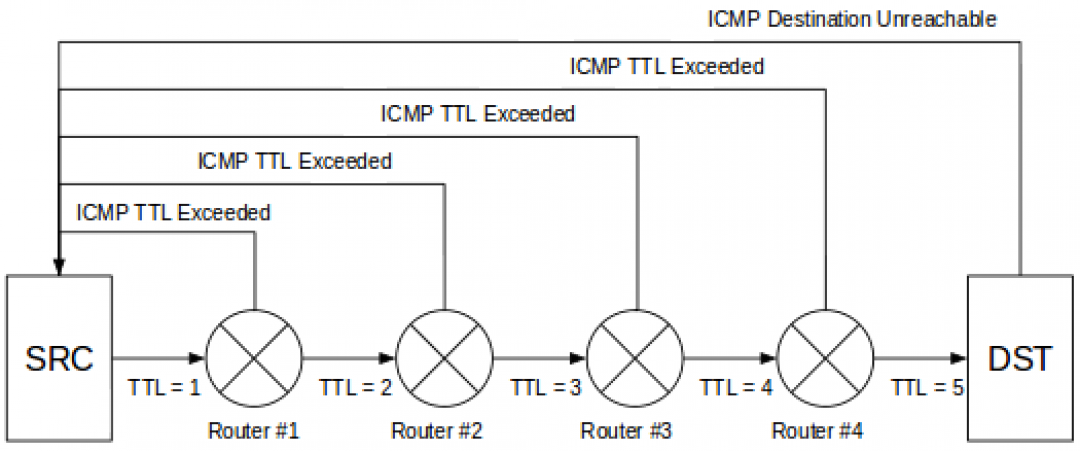
\includegraphics{traceroute-diagram.png}
    \caption{Diagram of how traceroutes work}
    \label{fig:traceroute_diagram}
\end{figure}

The mechanics of a traceroute program are then a very simple procedure. With $i=1$ to start, an \icmp-based traceroute program follows the below:

\begin{enumerate}
    \item Send an \icmp ping with \TTL$=i$ to the destination server.
    \item If an \icmp \ttl-expired packet is received, mark the sender as hop $i$ along the route. If a timeout is reached, skip.
    \item If an \icmp ping response is received (i.e. the destination was reached), mark the destination server as the $i$-th hop and note the time it took to receive the packet.
    \item Increment $i$ by one and repeat from step 1.
\end{enumerate}

This process produces a list of servers along the route and their associated \rtts. A sample output from the aptly-named \texttt{traceroute} utility\footnote{\texttt{traceroute} and its variations can be found on virtually every system made in recent memory. Linux distributions and Windows machines ship with command-line tools \texttt{traceroute} and \texttt{tracert} respectively, while MacOS has its own dedicated GUI application as a system tool.} is shown in \cref{fig:sample_traceroute}. The \texttt{* * *} instances on lines 2 and 10 indicate that no response was received from these hops, so \texttt{traceroute} proceeded without them.

\begin{code}
\centering
\begin{minipage}{0.33\textwidth}
    \begin{minted}{text}
 1  192.168.1.1  16.529 ms
 2  * * *
 3  96.34.83.9  26.158 ms
 4  96.34.84.212  30.452 ms
 5  96.34.2.142  31.084 ms
 6  96.34.0.51  31.012 ms
 7  96.34.0.137  27.184 ms
 8  96.34.3.89  23.049 ms
 9  96.34.148.35  28.703 ms
10  * * *
11  108.170.246.33  26.405 ms
12  108.170.246.34  24.091 ms
13  172.217.164.142 24.720 ms
    \end{minted}
\end{minipage}
    \caption{Truncated output from \texttt{traceroute google.com}}
    \label{fig:sample_traceroute}
\end{code}
